\chapter{Results}\label{chapter:results} \

In Chapter~\ref{chapter:results} we will introduce
the results of the experiments presented in Chapter
~\ref{chapter:implementation}. In Section~\ref{section:vqa_training}
we will present how the \ac{qml} models are trained.
Futhermore, in Section~\ref{section:vqa_attacks} the
attack methodology on the \ac{vqa} model will be described. \

\section{Iris Dataset}\label{section:iris-eval} \

\subsection{Noisy Models Accuracy}\label{subsection:iris-noisy-acc} \

\begin{figure}[!h]
  \centering

  \begin{subfigure}{0.45\textwidth}
      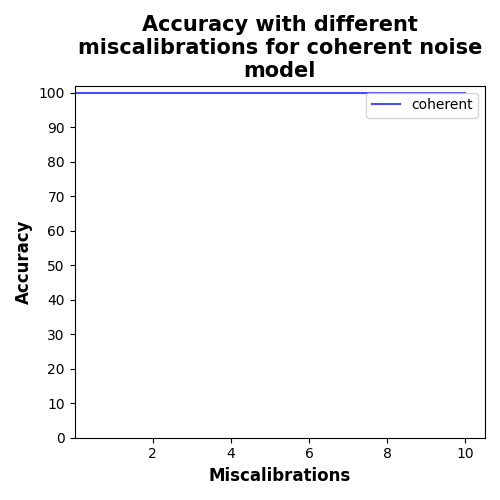
\includegraphics[width=\linewidth]{figures/evaluation_results/iris/pqc/figures/accuracy-coherent.png}
      \subcaption{Coherent noise model's accuracy.}
      \label{fig:iris1}
  \end{subfigure} \qquad
  \begin{subfigure}{0.45\textwidth}
      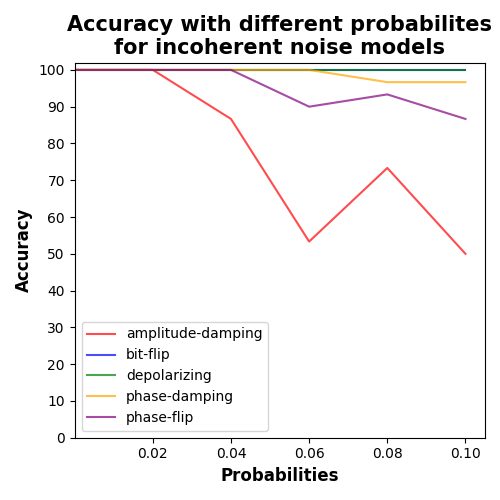
\includegraphics[width=\linewidth]{figures/evaluation_results/iris/pqc/figures/accuracy-incoherent.png}
      \subcaption{Incoherent noise models' accuracy.}
      \label{fig:iris2}
  \end{subfigure}

  \caption{\ac{vqa}'s accuracy on the Iris clean test dataset.}
\end{figure} \

\subsection{Adversarial Accuracy}\label{subsection:iris-adv-acc} \

\begin{figure}[!h]
  \centering

  \begin{subfigure}{0.45\textwidth}
      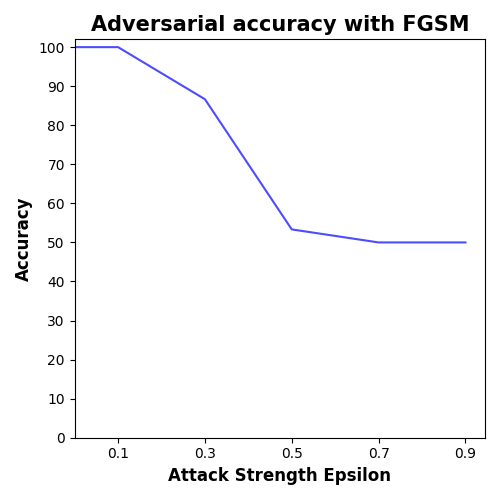
\includegraphics[width=\linewidth]{figures/evaluation_results/iris/pqc/figures/none-fgsm.png}
      \subcaption{Noiseless model's \ac{fgsm} adversarial accuracy.}
      \label{fig:iris3}
  \end{subfigure} \qquad
  \begin{subfigure}{0.45\textwidth}
      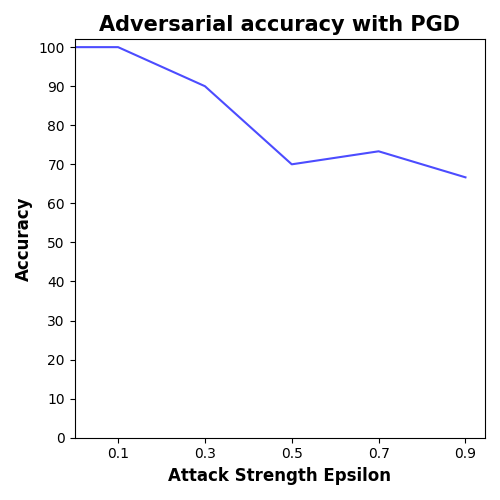
\includegraphics[width=\linewidth]{figures/evaluation_results/iris/pqc/figures/none-pgd.png}
      \subcaption{Noiseless model's \ac{pgd} adversarial accuracy.}
      \label{fig:iris4}
  \end{subfigure}

  \caption{\ac{vqa}'s accuracy on the adversarial Iris test dataset.}
\end{figure} \

\subsection{Noisy Models Adversarial Accuracy}\label{subsection:iris-noisy-adv-acc} \


\begin{figure}[!h]
  \centering

  \begin{subfigure}{0.45\textwidth}
      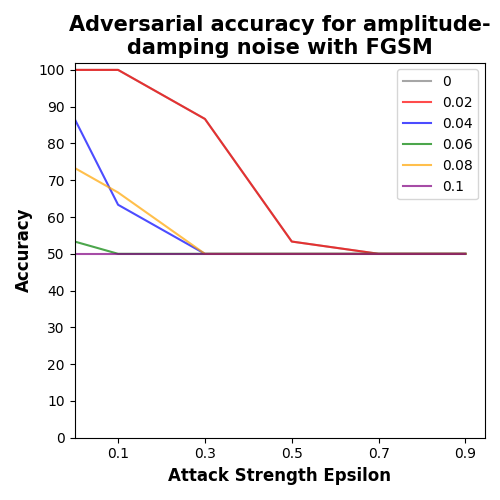
\includegraphics[width=\linewidth]{figures/evaluation_results/iris/pqc/figures/amplitude-damping-fgsm.png}
      \subcaption{Amplitude damping noise model's \ac{fgsm} adversarial accuracy.}
      \label{fig:iris5}
  \end{subfigure} \qquad
  \begin{subfigure}{0.45\textwidth}
      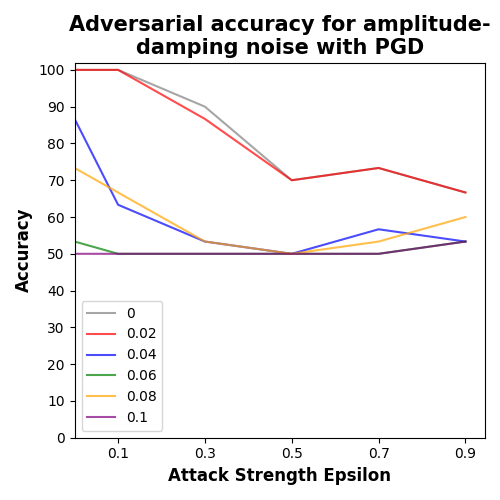
\includegraphics[width=\linewidth]{figures/evaluation_results/iris/pqc/figures/amplitude-damping-pgd.png}
      \subcaption{Amplitude damping noise model's \ac{pgd} adversarial accuracy.}
      \label{fig:iris6}
  \end{subfigure}

  \begin{subfigure}{0.45\textwidth}
      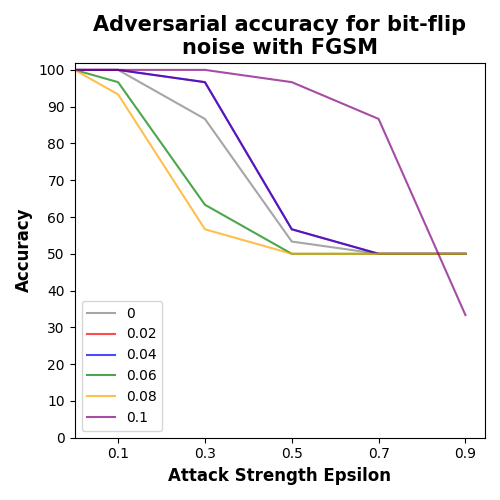
\includegraphics[width=\linewidth]{figures/evaluation_results/iris/pqc/figures/bit-flip-fgsm.png}
      \subcaption{Bit-Flip noise model's \ac{fgsm} adversarial accuracy.}
      \label{fig:iris7}
  \end{subfigure} \qquad
  \begin{subfigure}{0.45\textwidth}
      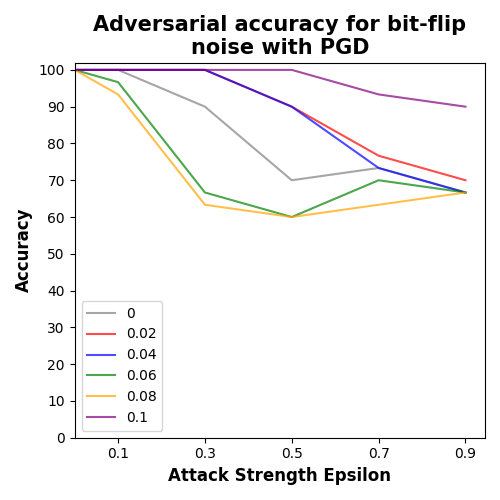
\includegraphics[width=\linewidth]{figures/evaluation_results/iris/pqc/figures/bit-flip-pgd.png}
      \subcaption{Bit-Flip noise model's \ac{pgd} adversarial accuracy.}
      \label{fig:iris8}
  \end{subfigure}

  \begin{subfigure}{0.45\textwidth}
      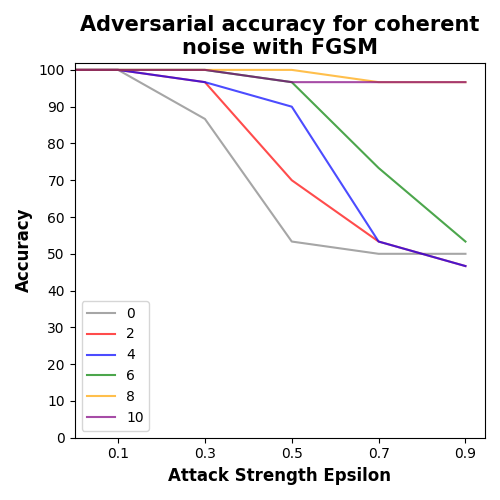
\includegraphics[width=\linewidth]{figures/evaluation_results/iris/pqc/figures/coherent-fgsm.png}
      \subcaption{Coherent noise model's \ac{fgsm} adversarial accuracy.}
      \label{fig:iris9}
  \end{subfigure} \qquad
  \begin{subfigure}{0.45\textwidth}
      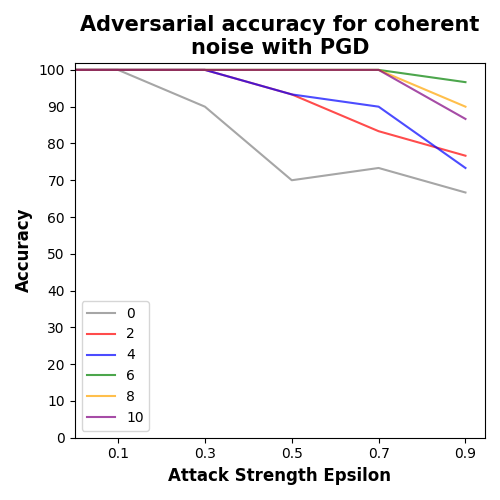
\includegraphics[width=\linewidth]{figures/evaluation_results/iris/pqc/figures/coherent-pgd.png}
      \subcaption{Coherent noise model's \ac{pgd} adversarial accuracy.}
      \label{fig:iris10}
  \end{subfigure}

  \begin{subfigure}{0.45\textwidth}
      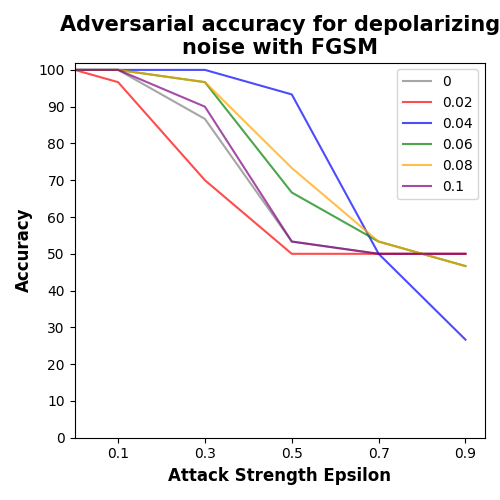
\includegraphics[width=\linewidth]{figures/evaluation_results/iris/pqc/figures/depolarizing-fgsm.png}
      \subcaption{Depolarizing noise model's \ac{fgsm} adversarial accuracy.}
      \label{fig:iris11}
  \end{subfigure} \qquad
  \begin{subfigure}{0.45\textwidth}
      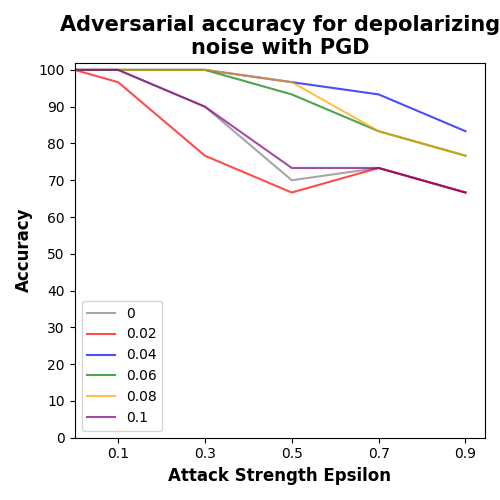
\includegraphics[width=\linewidth]{figures/evaluation_results/iris/pqc/figures/depolarizing-pgd.png}
      \subcaption{Depolarizing noise model's \ac{pgd} adversarial accuracy.}
      \label{fig:iris12}
  \end{subfigure}

  \begin{subfigure}{0.45\textwidth}
      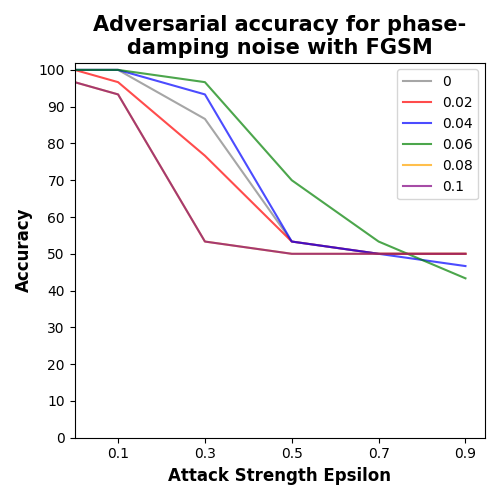
\includegraphics[width=\linewidth]{figures/evaluation_results/iris/pqc/figures/phase-damping-fgsm.png}
      \subcaption{Phase Damping noise model's \ac{fgsm} adversarial accuracy.}
      \label{fig:iris13}
  \end{subfigure} \qquad
  \begin{subfigure}{0.45\textwidth}
      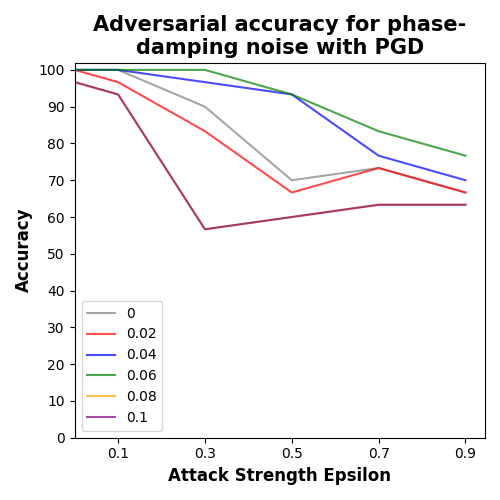
\includegraphics[width=\linewidth]{figures/evaluation_results/iris/pqc/figures/phase-damping-pgd.png}
      \subcaption{Phase Damping noise model's \ac{pgd} adversarial accuracy.}
      \label{fig:iris14}
  \end{subfigure}

  \begin{subfigure}{0.45\textwidth}
      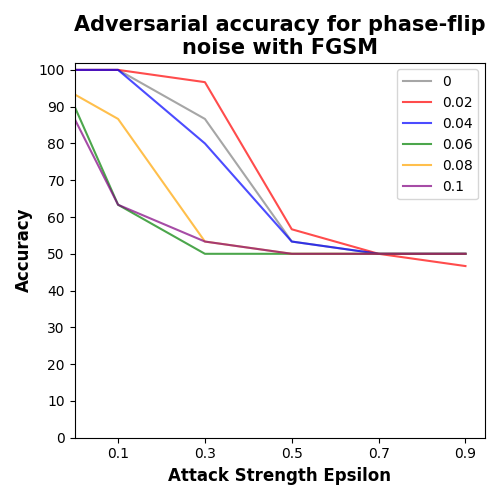
\includegraphics[width=\linewidth]{figures/evaluation_results/iris/pqc/figures/phase-flip-fgsm.png}
      \subcaption{Phase-Flip noise model's \ac{fgsm} adversarial accuracy.}
      \label{fig:iris15}
  \end{subfigure} \qquad
  \begin{subfigure}{0.45\textwidth}
      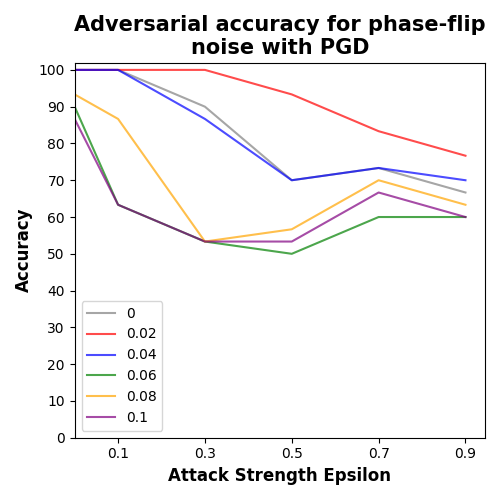
\includegraphics[width=\linewidth]{figures/evaluation_results/iris/pqc/figures/phase-flip-pgd.png}
      \subcaption{Phase-Flip noise model's \ac{pgd} adversarial accuracy.}
      \label{fig:iris16}
  \end{subfigure}

  \caption{Noisy models' accuracy on the adversarial Iris test dataset.}
\end{figure} \

\section{\acl{pid} Dataset}\label{section:diabetes-eval} \

\subsection{Noisy Models Accuracy}\label{subsection:diabetes-noisy-acc} \

\subsection{Adversarial Accuracy}\label{subsection:diabetes-adv-acc} \

\subsection{Noisy Models Adversarial Accuracy}\label{subsection:diabetes-noisy-adv-acc} \

\section{Breast Cancer Dataset}\label{section:breast-cancer-eval} \

\subsection{Noisy Models Accuracy}\label{subsection:breast-cancer-noisy-acc} \

\subsection{Adversarial Accuracy}\label{subsection:breast-cancer-adv-acc} \

\subsection{Noisy Models Adversarial Accuracy}\label{subsection:breast-cancer-noisy-adv-acc} \

\section{Plus-Minus Dataset}\label{section:plus-minus-cancer-eval} \

\subsection{Noisy Models Accuracy}\label{subsection:plus-minus-cancer-noisy-acc} \

\subsection{Adversarial Accuracy}\label{subsection:plus-minus-cancer-adv-acc} \

\subsection{Noisy Models Adversarial Accuracy}\label{subsection:plus-minus-cancer-noisy-adv-acc} \


1.	Explain why decoherent noise is used and not coherent. \

  a. Coherent noise will probably just shift the bias. \

  b. Coherent noise might add too much noise (quadratic growth). \

  c. True random noise is required to improve generalization. \

% TODO: Do an experiment implementing coherent noise to prove this claim.
% Use https://pennylane.ai/qml/demos/tutorial_variational_classifier/ - circuit-centric quantum classifier ansatz

\section{Variational Quantum Algorithm Model Accuracy}\label{section:vqa_accuracy} \

% TODO: State the result of training QVC with regards to the chosen datasets.
% TODO: Compare to paper and state why they might be valid results.

\section{Variational Quantum Algorithm Model Adversarial Accuracy}\label{section:vqa_adversarial_accuracy} \

% TODO: Present results per dataset of the different attacks and attack strengths